\section{Wiktor Prosowicz}{\centering}

My favourite mathematical expression is so called "Piwo equation" : \\
\(P^2 + I*W*O =  :-)\)

\vspace{1cm}
\begin{quote}{\small}
    The most important mathematical thesis can be described as \\
    \(\sqrt{PIWO} + \sqrt{sok} = :-(\) -- Socrates
\end{quote}
\vspace{2cm}

This is my favourite kind of beverage:
\begin{figure}[htbp]
    \centering
    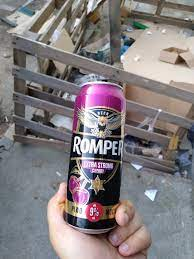
\includegraphics[scale=0.6]{Pictures/5_WProsowicz_romperek.jpg}
    \caption{Romperek mmmmmm pyszny}
    \label{fig:romper}
\end{figure}
\vspace{1cm}

\setlength{\parindent}{10ex}
 \textbf{ Następny wynalazek grupy CO, dostępny w sieci Żabka. Najprawdopodobniej następca Roger's Strong, szata graficzna puszki ta sama, tylko nazwa piwa zmieniona. Czy to produkt browaru z Brzeska, to sobie głowy uciąć nie dam, bo podany tylko adres warszawski grupy.
Zawartość alk. 6,2% obj., ekstraktu nie podano, cena niecałe 2 złote.
Piana obfita przez krótka chwilę, gaz w normie, jak na stronga, to tej mocy nie czuć. Piwo na \underline{spróbowanie}}.\par
\vspace{0.5cm}

\setlength{\parindent}{10ex}
 \textit{Właśnie popijam Rompera Strong. Zapach lekko chmielowy.Piana zniknęła w mgnieniu oka. Wysycenie całkiem przyzwoite. Barwa jasno miodowa. W smaku czuć alkohol oraz goryczkę. Ogólnie jednak wodnisty. Nie polecam. Moja ocena 2-.}
 \par
\vspace{1.0 cm}

\centering
\begin{table}[htbp]
\centering
\begin{tabular}{|l|l|l|ll}
\cline{1-3}
\cellcolor[HTML]{FFCCC9}{\color[HTML]{333333} \textbf{Nazwa}} & \cellcolor[HTML]{FFCCC9}{\color[HTML]{333333} \textbf{Ocena}} & \cellcolor[HTML]{FFCCC9}{\color[HTML]{333333} \textbf{Cena}} &  &  \\ \cline{1-3}
Romper Extra Strong                                           & 5.0                                                           & 3 zł                                                         &  &  \\ \cline{1-3}
Kuflowe Mocne                                                 & 4.0                                                           & 2.5 zł                                                       &  &  \\ \cline{1-3}
Wódeczka Soplica                                              & 4.5                                                           & 24 zł                                                        &  &  \\ \cline{1-3}
\end{tabular}
\label{tab:piwa}
\end{table}
--Table containing drinks that are always good
\par
\vspace{1cm}

List of project I'm working on
\begin{enumerate}
  \item Flashcard App
  \item HTML Parser
  \item Chinese characters database management app
\end{enumerate}
\vspace{1cm}

List of my planned projects
\begin{itemize}
\renewcommand{\labelitemi}{$*$}
    \item Website
    \item Online game
\end{itemize}
\vspace{1cm}

\raggedleft
Here you can return to my image: Image nr ~\ref{fig:romper} \\
And here to my table: Table nr ~\ref{tab:piwa}


